\documentclass[10pt,a4paper,twocolumn]{article}

\usepackage[a4paper,margin=2cm,columnsep=0.7cm]{geometry}

\usepackage{fontspec}
\setmainfont{texgyretermes}[Path=fonts/, Extension=.otf, UprightFont=*-regular, BoldFont=*-bold, ItalicFont=*-italic, BoldItalicFont=*-bolditalic]
\usepackage{amsmath}
\usepackage{booktabs}
\usepackage[table]{xcolor}
\usepackage{tikz}
\usepackage{titlesec}
\usepackage{ragged2e}
\usepackage{url}

\definecolor{accent}{HTML}{000000}

\titleformat{\section}
  {\color{accent}\bfseries\large}{\thesection.}{0.5em}{}
\titleformat{\subsection}
  {\color{accent}\bfseries\normalsize}{\thesubsection}{0.5em}{}
\titlespacing*{\section}{0pt}{1.4ex plus .2ex}{0.3ex}

\setlength{\parindent}{0pt}
\setlength{\parskip}{0.5em}

\title{\vspace{-1.5em}\bfseries\color{accent}\Large Foundations of a Personal Finance System: The Three Pillars}
\author{}
\date{}

\begin{document}

\twocolumn[
  \begin{@twocolumnfalse}
    \maketitle
    \vspace{-3.8em}
    \begin{center}
      \small Nonthawit Doungsodsri\\
      nonthawit.com\\
      3 June 2026\\
      Version 1.0.0
    \end{center}
    \vspace{0.5em}
    \begin{quote}
      \normalsize\textbf{Abstract} --- This paper presents a simple yet durable framework for building personal finances, the ``Three-Pillar System'': Cashflow Management (Cashflow), Investment, and Savings (value preservation). Its central claim is that long-term financial success does not come from sophisticated strategy, but from \textbf{discipline} and following your own system consistently for five to ten years or more.
    \end{quote}
    \vspace{1em}
  \end{@twocolumnfalse}
]

\section{Introduction}
Personal finance is the management of one's own money in line with one's life goals. For most people the problem is not earning too little, but lacking a clear \textit{system} for managing the money they make. This paper offers a tangible system usable for a lifetime, resting on a single foundational equation.

\begin{center}
{\setlength{\fboxsep}{10pt}\fbox{$\displaystyle \text{Income} \;-\; \text{Expenses} \;=\; \text{Freedom Fund}$}}
\end{center}

The ``Freedom Fund'' is the raw material of financial freedom. If the result is negative, the first goal is to turn it positive. If it is positive, the next question is how to allocate it. This paper's answer is to channel the Freedom Fund into three pillars that work together: Cashflow Management, Investment, and Savings. Each pillar has its own role and goal, explained in turn below.

\section{Pillar 1 --- Cashflow Management}
\textbf{What it is.} Cashflow management means knowing how much money flows in and out each month, by recording income and expenses consistently. No complex tools are required; a simple notebook or app is enough. The key is continuity, not sophistication.

\textbf{Goal.} To know your true ``Freedom Fund'' each month, the number that tells you how much capacity you have to invest and save. Without it, every plan is a guess. This pillar is the \textit{foundation} the other pillars stand on.

\textbf{Practice.} Record daily or weekly until it becomes a habit, review your month-end totals, separate essential spending from discretionary spending, and aim to keep the ``Freedom Fund'' firmly positive before moving on to the second and third pillars.

\section{Pillar 2 --- Investment}
\textbf{What it is.} Investment means putting your money to work for you, channeling the Freedom Fund into long-term returns. Unlike holding idle cash, invested money has the chance to grow through compounding over time.

\textbf{Goal.} To generate returns that grow wealth faster than saving alone and bring you closer to financial freedom. The key principle is to \textbf{invest only in what you thoroughly understand}. Investing by hype, without understanding the asset, opens the door to uncontrollable risk.

\textbf{Practice.} Do not rush; investing is like planting a tree, you cannot force it to grow. Begin by studying until you understand, then use \textbf{DCA} (Dollar-Cost Averaging): buying assets steadily every month regardless of price swings. This removes emotion from decisions and builds durable investing discipline, ideal for beginners. That said, DCA is only one of many ways to start investing. Other approaches exist, such as lump-sum investing, rebalancing, or value investing; each has its own strengths and suits different situations. Readers should study and choose the method that fits their goals and temperament.

\section{Pillar 3 --- Savings (Value Preservation)}
\textbf{What it is.} Saving here does not mean piling up idle cash, but holding \textbf{value-preserving assets} to reduce life's risks. Cash left idle loses purchasing power every year to inflation; good saving must protect the value of your money from erosion.

\textbf{Goal.} To build security and a buffer against risk, so that when the unexpected happens you have assets that retain their value to rely on. This pillar plays ``defense'' while the investment pillar plays ``offense''.

\textbf{Practice.} Rather than fixating on any single asset, choose by the \textbf{qualities} that preserve value well, such as resistance to inflation, reasonable liquidity, and broad acceptance. Present-day examples include gold, index funds, bonds, or insurance to transfer risk, all of which may change with the times. Readers should therefore study the options available at the time, diversify so that risk is not concentrated in one asset, and maintain a steady savings rate just as with investing.

\section{Allocation and Discipline}
Once you understand the three pillars, the practical question is how to divide the ``Freedom Fund'' among them. The three pillars are not separate; they work together to support a single goal, financial freedom, as shown in Figure~\ref{fig:pillars}.

\begin{figure}[t]
\centering
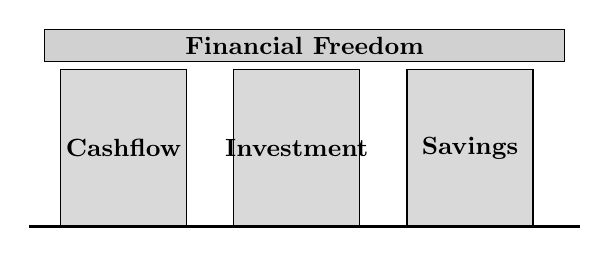
\begin{tikzpicture}[font=\small]
  \fill[accent!18] (-0.2,2.1) rectangle (6.4,2.5);
  \draw[accent] (-0.2,2.1) rectangle (6.4,2.5);
  \node[accent] at (3.1,2.3) {\bfseries Financial Freedom};
  \foreach \x/\lbl in {0/Cashflow, 2.2/Investment, 4.4/Savings} {
    \fill[accent!15] (\x,0) rectangle (\x+1.6,2.0);
    \draw[accent] (\x,0) rectangle (\x+1.6,2.0);
    \node[accent,align=center] at (\x+0.8,1.0) {\bfseries \lbl};
  }
  \draw[accent,line width=1pt] (-0.4,0) -- (6.6,0);
\end{tikzpicture}
\caption{The three pillars supporting financial freedom.}
\label{fig:pillars}
\end{figure}

\textbf{Example allocation.} Suppose an income of \$2{,}500 per month with \$1{,}500 in essential expenses, leaving \$1{,}000 as the Freedom Fund. We can split this Freedom Fund 30/40/30 as in Table~\ref{tab:alloc}. What must be stressed is that the 30/40/30 figures are only an illustrative example, not a formula. Each person has different income, obligations, goals, and risk tolerance; a ratio that suits one person may not suit another. Readers should design their own ratio from their real situation. What cannot be omitted is that the Freedom Fund must always flow into the \textbf{Investment} and \textbf{Savings} pillars; these two are mandatory and every plan must include them. How large the proportions are, and how the remainder (such as discretionary spending or other goals) is allocated, readers may design freely to fit their own lives.

\begin{table}[t]
\centering
\small
\begin{tabular}{lrr}
\toprule
\rowcolor{accent!15}
\textbf{Destination} & \textbf{Share} & \textbf{Amount (USD)} \\
\midrule
Investment   & 30\% & \$300 \\
Savings      & 40\% & \$400 \\
Discretionary & 30\% & \$300 \\
\midrule
\textbf{Total Freedom Fund} & \textbf{100\%} & \textbf{\$1{,}000} \\
\bottomrule
\end{tabular}
\caption{Example allocation of a \$1{,}000 Freedom Fund (illustrative).}
\label{tab:alloc}
\end{table}

\textbf{Discipline is the heart.} However you allocate, the deciding factor of success is not the ratios or any complex strategy, but \textbf{following your own system consistently for five to ten years or more}. The power of DCA and continuous saving becomes clear only when you let time and compounding do their work. The deepest benefit of having a system is that it dampens the influence of emotion, both greed in rising markets and fear in volatile ones, the true enemies of long-term finances. When you follow the system, decisions rest on principle, not momentary feeling. Those who start early and stay consistent will always beat those who are clever but start and stop.

\section{Conclusion}
Building solid personal finances requires no advanced financial knowledge or secret strategy, only a system that is easy to understand and discipline that is actually doable. The three pillars --- cashflow management to know your Freedom Fund, investment to put money to work for you, and savings to reduce risk --- when worked together consistently, gradually raise the quality of your financial life all along the way.

The principle to carry with you is: \textbf{``Start with a simple system, then do it consistently.''} Time and consistency are every investor's most powerful allies.

\vspace{1em}
\noindent\rule{\linewidth}{0.4pt}\\
{\small\raggedright This document is the work of \textbf{Nonthawit Doungsodsri} --- released for the public good. Learn more at nonthawit.com\par}

\end{document}
